\chapter{Clustering}


\section{Clustering within classes using PCA}
We decided to first try see if any of the digits would get separated using a PCA. We found that the digit 3 and 5 was somehow separated into two classes with a few intermediate clusters.

\begin{figure}[H]
\centering
\includegraphics[width=1\linewidth]{code/pca_digit_cluster}
\caption{}
\label{fig:pca_cluster}
\end{figure}

In both cases this turned out to be a separation of whether the digits was bold or thin. In figure~\ref{fig:pca_cluster} the clusters can be seen separated by a low density region in the middle. We made the same plot with larger digits to show what meaning the PCA components had, but this means the clusters fade due to spacing between the digits. You can always open the PDF to inspect the numbers.

\begin{figure}[H]
\centering
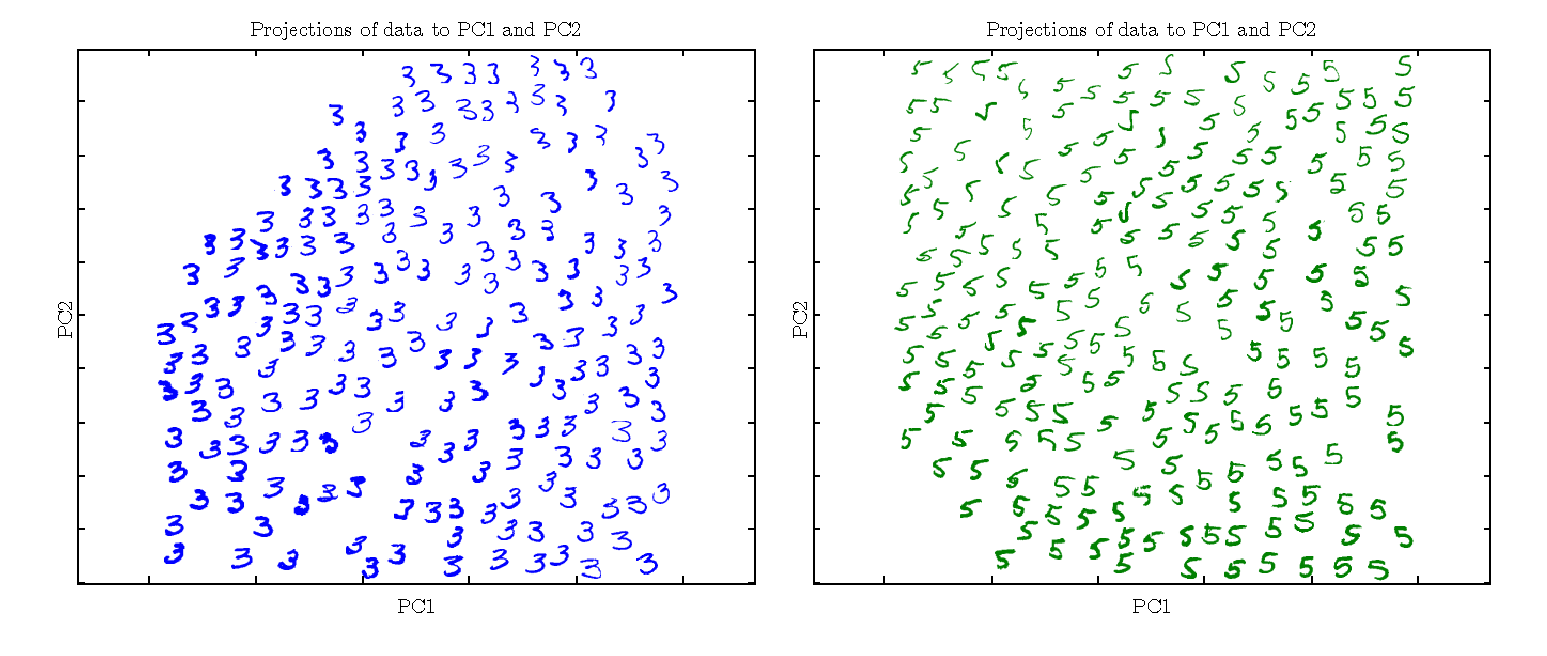
\includegraphics[width=1\linewidth]{code/pca_digit_cluster_z}
\caption{}
\label{fig:pca_cluster_zoom}
\end{figure}


\section{Gaussian Mixture Model (GMM) cross-validation}

As asked in the assignment we have clustered our data by the Gaussian Mixture Model and used cross-validation to determine the how many clusters produces the best results. \\

Since our data set (again) is too big such that we are unable to run this in a decent time, we have had to take some measures to bring the run-time down. As such we have decided to use the 40 first principal components from a PCA over the digits, instead of the 272 original attributes. We have also cut the observation size down from 60.000 to 10.000, and even with all this it is still incredibly compute heavy and takes ages to run. \\

The result using different amount of clusters ($K$) is shown below.

\begin{figure}[H]
\centering
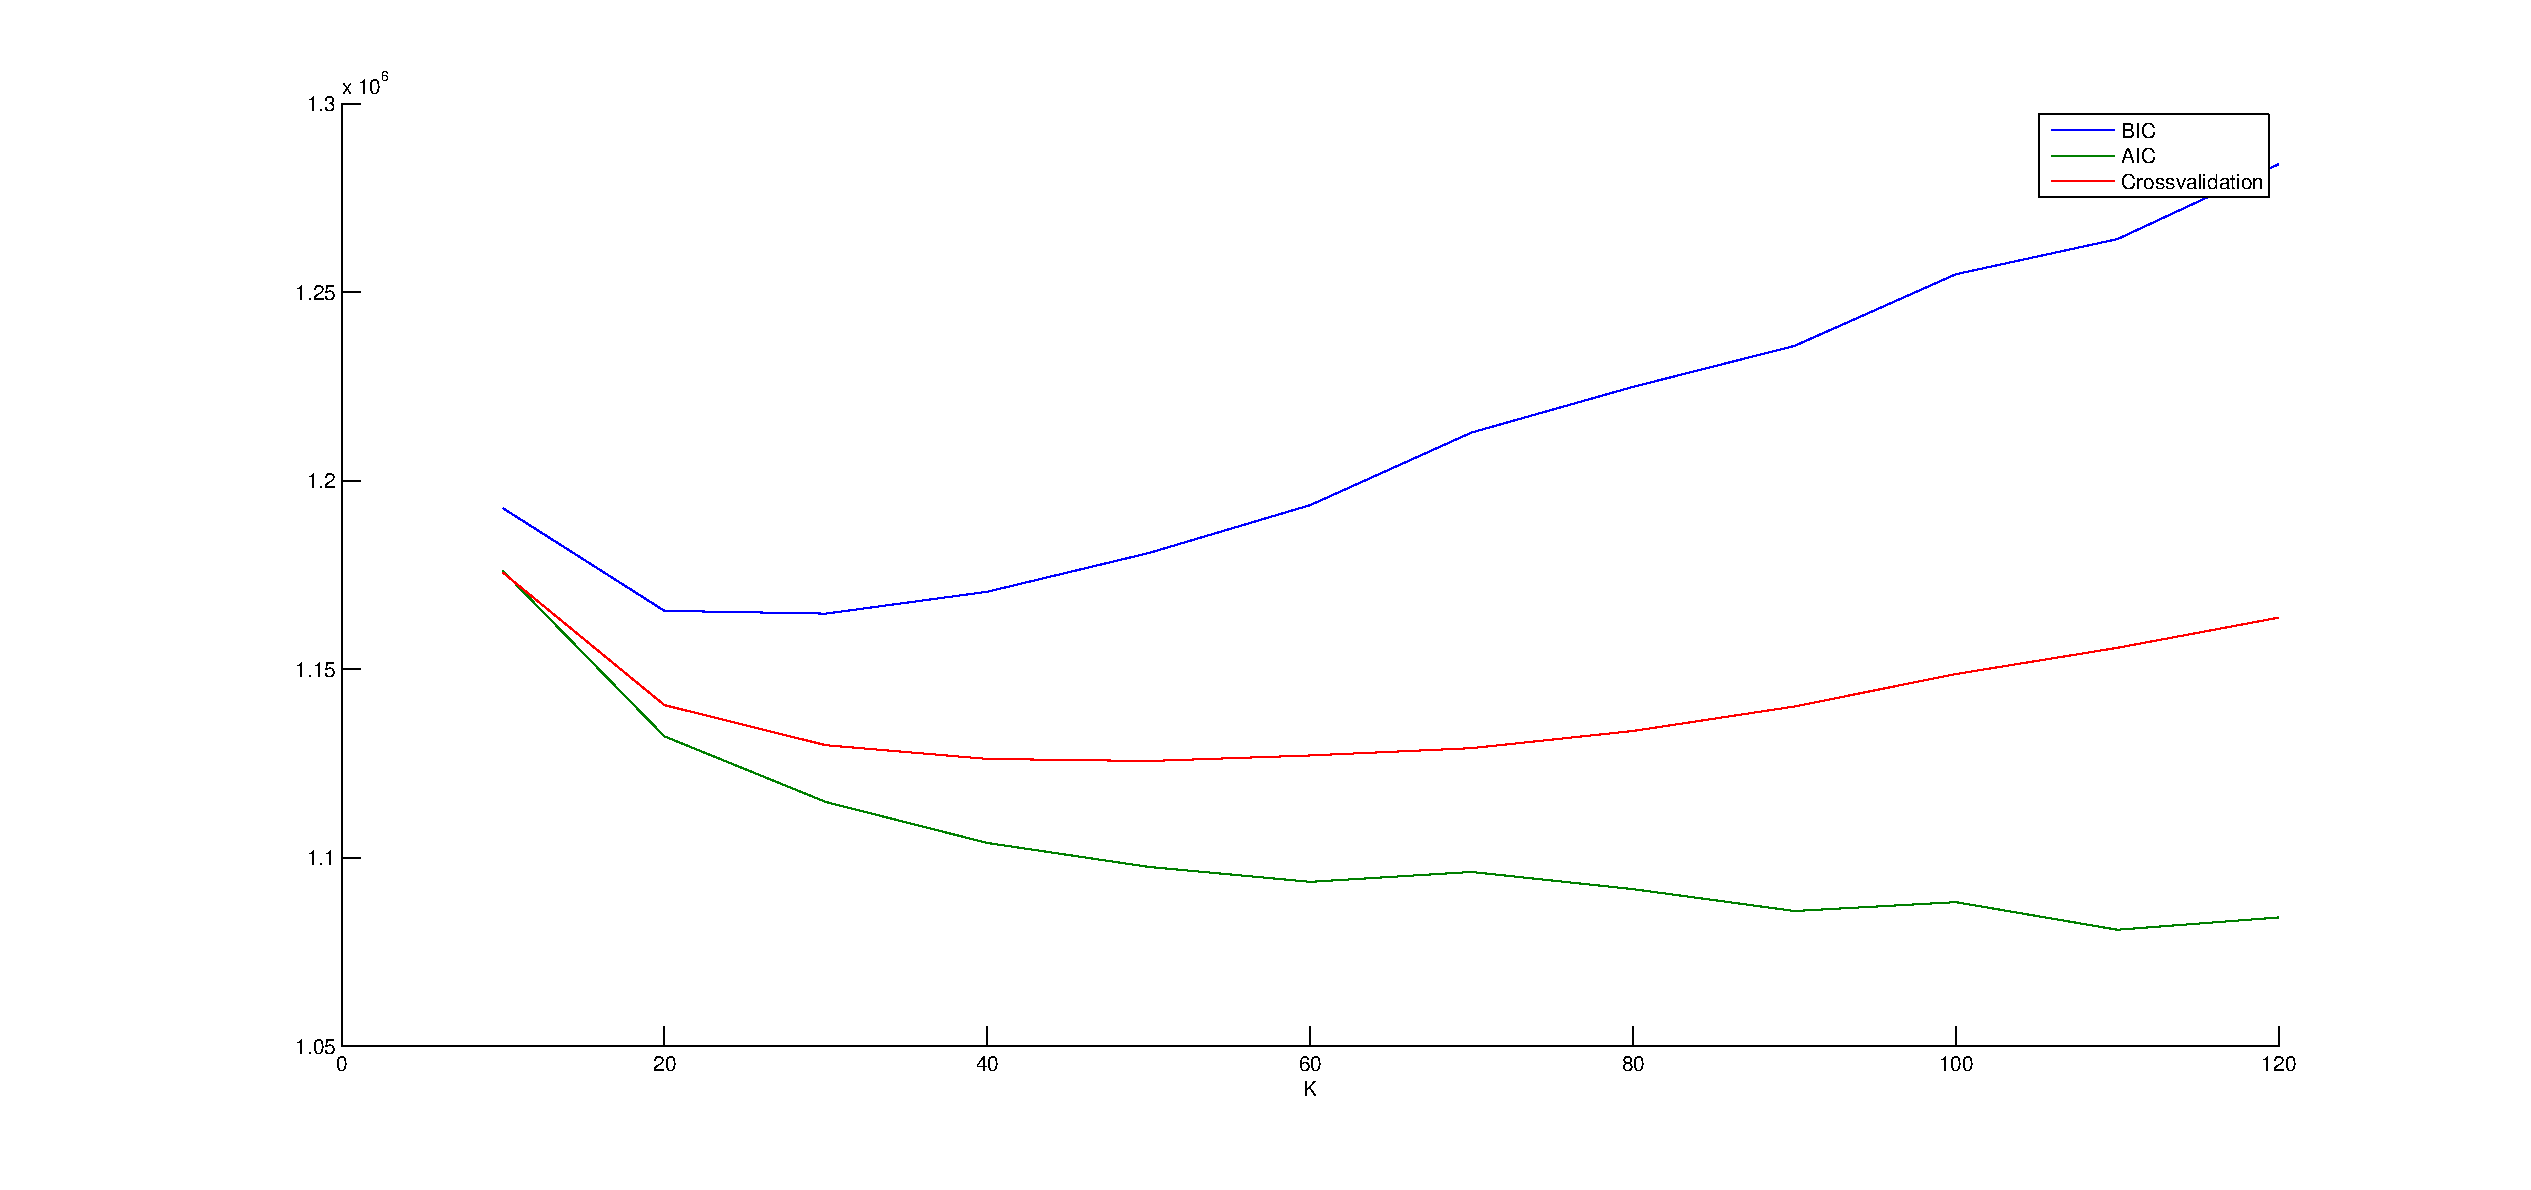
\includegraphics[width=1\linewidth]{code/pca_gmm10-120_cv}
\caption{The y-axis is the negative logarithm-likelihood for each amount of clusters $K$. Besides cross-validation, AIC and BIC are also plotted on the graph. One can see that the maximum likelihood is around K=50 for CV.}
\label{fig:pca_gmm10-120_cv}
\end{figure}


From this we can conclude that when using this clustering method with cross-validation on all 10 of our digits, we need to use 50 clusters to get the best result. 

The centers for the clusters do not hold any significant meaning because of the nature of the data set, which is why we have not done any further analysis on this. \\

A GMM run-through (replicates 10) with 50 clusters gave an average success rate for the clusters of $82.9\%$ of getting the the mode of the cluster (the most frequent class in the cluster).

\section{Hierarchical clustering}

Every time we try to run the functions to do any hierarchical clustering it errors out because of too high recursion or some indexing errors. It seems that it is simply too much data for the function(s) to handle, and because of that we have not been able to get any result using this clustering technique.


\section{GMM with matching amount of clusters}

To test for actual clusters which correspond to our digit classes in the data set we set out to use exactly the amount of clusters needed depending on how many classes were used. First off we started with the digits 0 and 1, and using only the first 10 principal components we got the following clustering from GMM:

\begin{figure}[H]
\centering
\includegraphics[width=1\linewidth]{code/gmm_0-1}
\caption{Clustering of the digits 0 and 1 shown using the two first principal components.}
\label{fig:gmm_0-1}
\end{figure}

\begin{verbatim}
Cluster 1 has mode 0. Success rate: 5922/6081 (97.3853%)
Cluster 2 has mode 1. Success rate: 6583/6584 (99.9848%)
OVERALL: 98.7367%
\end{verbatim}

A pretty good success rate, and it can be seen from the plot that the two first PCs split the two digit classes pretty well, which makes it ideal for clustering. \\

Following this we continued with more digits classes and clusters. Following $K=3$ GMM clustering with an extra digit, namely 2. Again we used only the 10 first principal components to get this clustering and success rate:

\begin{figure}[H]
\centering
\includegraphics[width=1\linewidth]{code/gmm_0-2}
\caption{Clustering of the digits 0, 1 and 2 shown using the two first principal components.}
\label{fig:gmm_0-2}
\end{figure}

\begin{verbatim}
Cluster 1 has mode 0. Success rate: 5679/5693 (99.7541%)
Cluster 2 has mode 1. Success rate: 6365/6365 (100.0000%)
Cluster 3 has mode 2. Success rate: 5944/6565 (90.5407%)
OVERALL: 96.5902%
\end{verbatim}

\vspace{1cm}

Finally we attempted with all 10 digits and 40 PCs instead of just 10 in order to achieve a better result. This is the result of doing it with 40 PCs:

\begin{verbatim}
Cluster 1 has mode 6. Success rate: 5102/5137 (99.3187%)
Cluster 2 has mode 4. Success rate: 5310/6164 (86.1454%)
Cluster 3 has mode 8. Success rate: 2208/6233 (35.4244%)
Cluster 4 has mode 1. Success rate: 5934/5939 (99.9158%)
Cluster 5 has mode 0. Success rate: 5131/5147 (99.6891%)
Cluster 6 has mode 2. Success rate: 4117/5503 (74.8137%)
Cluster 7 has mode 8. Success rate: 3052/8561 (35.6500%)
Cluster 8 has mode 9. Success rate: 4416/4633 (95.3162%)
Cluster 9 has mode 3. Success rate: 2440/7871 (30.9999%)
Cluster 10 has mode 7. Success rate: 4711/4812 (97.9011%)
OVERALL: 70.7017%
\end{verbatim}

The plot with PC1/PC2 is just one big glob where nothing is distinguishable, so we have left it out. From the above results we can see that some clusters capture a single class very well, namely cluster 1, 4, 5, 8 and 10 are all above $95\%$. This means that we are pretty good at determining the class of an observation in those areas. The rest seems to be a worse mixture of classes which 10 clusters are not good at distinguishing.

Using 50 clusters from the cross-validation part of this chapter had a better success rate, but still not a super good one.
